

\documentclass{beamer}
% \usetheme{Boadilla}


\title{ANNs in Feedback Paths for novel Audio Effects}
% \subtitle{Exploration of Neural Networks in fe}
\author{Patrik Lechner\texorpdfstring{\\}{,} }
% \titlegraphic{\includegraphics[scale=1.25]{focuslogo.pdf}}
\institute{IC\textbackslash M/T \\ FH Stp.}
\date{June 19 2020}

% ==========THEME=====================
\usetheme{Warsaw}

\setbeamercolor{normal text}{fg=white,bg=black!90}
\setbeamercolor{structure}{fg=white}

\setbeamercolor{alerted text}{fg=red!85!black}

\setbeamercolor{item projected}{use=item,fg=black,bg=item.fg!35}

\setbeamercolor*{palette primary}{use=structure,fg=structure.fg}
\setbeamercolor*{palette secondary}{use=structure,fg=structure.fg!95!black}
\setbeamercolor*{palette tertiary}{use=structure,fg=structure.fg!90!black}
\setbeamercolor*{palette quaternary}{use=structure,fg=structure.fg!95!black,bg=black!80}

\setbeamercolor*{framesubtitle}{fg=white}

\setbeamercolor*{block title}{parent=structure,bg=black!60}
\setbeamercolor*{block body}{fg=black,bg=black!10}
\setbeamercolor*{block title alerted}{parent=alerted text,bg=black!15}
\setbeamercolor*{block title example}{parent=example text,bg=black!15}
% ==========THEME=====================

% =========TIKZ=============
\usepackage{tikz}
\usetikzlibrary{dsp,chains}

\DeclareMathAlphabet{\mathpzc}{OT1}{pzc}{m}{it}
\newcommand{\z}{\mathpzc{z}}

\usepackage[skins]{tcolorbox}

% Definition of blocks:
\tikzset{%
  block/.style    = {draw, thick, rectangle, minimum height = 3em,
    minimum width = 3em},
  sum/.style      = {draw, circle, node distance = 2cm}, % Adder
  input/.style    = {coordinate}, % Input
  output/.style   = {coordinate}, % Output
  mult/.style	  = {draw, isosceles triangle, minimum height=1cm, minimum width =1cm}
}


% tikz image

\usepackage{mwe}
\tikzset{
  path image/.style={
    path picture={
      \node at (path picture bounding box.center) {
		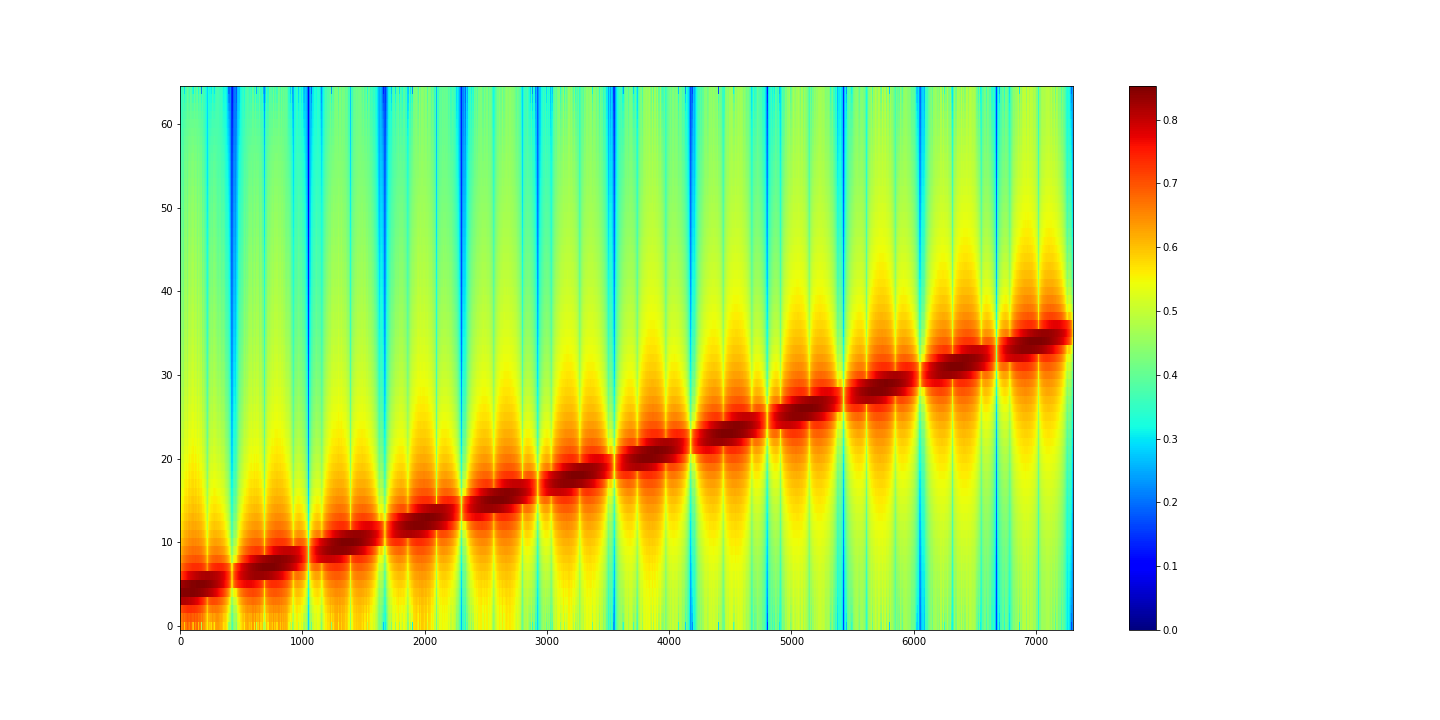
\includegraphics[height=5cm]{modSweep.png}};}},
	path yimage/.style={
			path picture={
			  \node at (path picture bounding box.center) {
				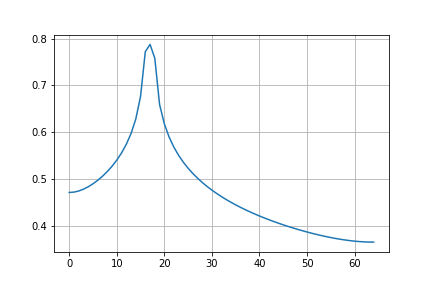
\includegraphics[height=2.5cm]{oneY.png}};}},
  path tikzimage/.style={
    path picture={
      \node at (path picture bounding box.center)
        [circle, fill=blue!50, scale=2, text=yellow]{Bravo};}}
}


% ==========================

% ======audio=====]
\usepackage{media9}




\usefonttheme[onlymath]{serif}

\begin{document}

    \begin{frame}
		\maketitle
		
		https://github.com/hrtlacek/audioFeedbackNN
    \end{frame}
    
	\section{Concept}
	
    \begin{frame}{Background}
    	The presented system was built around the following ideas:
    	\begin{itemize}
        \item Create an expressive system that can be used by artists in the field of experimental electronic music
        \item Use AI to autgenerate content but give control to the artist
        \item achieve aesthetical results that are directly useful/interesting on their own
		\item exploit neural network specific artifacts as novel timbres
		\item Create an architecture with the possibility of real time execution in mind
        \end{itemize} 
    \end{frame}


	\begin{frame}
		A Network, $G$ is trained to predict Short-Time Fourier Transform (STFT) Frames, $X[n]$ given $k$ number of 
		past STFT frames so that it ideally satisfies:
		
		\begin{equation}
			G\{X[m-1, \omega],..., X[m-k, \omega]\}=X[m, \omega]
		\end{equation}

		The training data for the network can be chosen at will and has great influence on the aesthetical result. 
		

	\end{frame}

	\begin{frame}{Example}
		\centering
		% \noindent
		\begin{tikzpicture}
			% \path[fill overzoom image=modSweep.png] (0,0) rectangle (\textwidth,2cm);
			\draw [path image,draw=blue,thick] (2,0) rectangle +(5,3);
			\draw [path image,draw=blue,thick] (2,-3) rectangle +(0.5,2);
			\node [dspsquare](g) at (3.7,-2.){$G$};
			\draw [path yimage,draw=blue,thick] (5,-3) rectangle +(2,2);

			\node[draw, rectangle,white, thick, line width=1mm,minimum height=3.2cm, minimum width =0.5cm](fr) at (2.5,1.5) {};
			\node[draw, rectangle, white,thick, line width=1mm,minimum height=3.2cm, minimum width =0.001cm](fr) at (3,1.5) {};

			\node[coordinate](xds) at (2.5,-0.1) {};
			\node[coordinate](xdi) at (2.5,-0.5) {};

			\node[coordinate](xdi2) at (2.25,-1) {};

			\node[coordinate](yds) at (3,-0.1) {};

			\node[coordinate](ydi) at (3.,-0.5) {};

			\node[coordinate](ydi2) at (5.25,-1) {};

			\node[coordinate](xd) at (2.5,-2) {};
			\node[coordinate](y) at (5,-2) {};

			\draw[dspflow] (xds) -- (xdi);
			\draw[dspconn] (xdi) -| (xdi2);

			\draw[dspflow] (yds) -- (ydi);
			\draw[dspconn] (ydi) -| (ydi2);



			\draw[dspconn] (xd) -- (g);
			\draw[dspconn] (g) -- (y);

			% \draw (0,0) rectangle (2,2) node[pos=.0] {Test};
			\node[draw, text width=6.8cm] (bla) at(4.5,3.5) {Source Data (amp modulated sine sweep)};
			


		\end{tikzpicture}
		
	\end{frame}


	\begin{frame}{Architecture}
	Theoretically, such a network should be able to completely reproduce the training data by itself if fed back its buffered 
	output and the buffer being initialized with the beginning of the training set:
		 
		\vspace{1cm}

    \centering
	\begin{tikzpicture}
	[align=center,node distance=1.2cm]
	\node[coordinate,dsp/label=right] (c0) {};

	\node[dspsquare, right of= c0] (buf) {$buf$};

	\node[dspsquare, right of=buf] (AI) {$ANN$};

	\node[dspnodeopen, right of=AI]  (split) {};

	\node[dspsquare, right of=split] (istft) {$\mathcal{F}^{-1}$};

	\node[dspnodeopen, right of=istft]  (outp) {$y[n]$};

	\node[coordinate,dsp/label=right, below of=c0] (c1) {};

	\draw[dspconn] (AI) -- (istft);
	\draw[dspconn] (c1) |- (buf);
	\draw[dspconn] (istft) -- (outp);
	\draw[dspconn] (buf) -- (AI);

	\draw[dspflow] (split) |- (c1);

	\end{tikzpicture}

	\end{frame}




	\begin{frame}{Architecture}
		This brings the opportunity to feed in an additional fourier transformed 
		 time 
		domain signal which can be used to control the networks 
		tendency which parts of the trainingset to reproduce. 
		 
		\vspace{1cm}

    \centering
	\begin{tikzpicture}
		[align=center,node distance=1.2cm]
	\node[dspnodeopen,dsp/label=left]  (inp) {$x[n]$};	
    % \node[dspnodeopen] (m13) {};
	\node[dspsquare, right of=inp] (stft){$\mathcal{F}$};

	\node[dspadder, right of=stft] (add1) {};

	\node[dspsquare, right of=add1] (buf) {$buf$};

	\node[dspsquare, right of=buf] (AI) {$ANN$};

	\node[dspnodeopen, right of=AI]  (split) {};

	\node[dspsquare, right of=split] (istft) {$\mathcal{F}^{-1}$};

	\node[dspnodeopen, right of=istft]  (outp) {$y[n]$};


	\node[coordinate,dsp/label=right, below of=add1]                  (c1) {};


	\draw[dspconn] (inp) -- (stft);
	\draw[dspconn] (stft) -- (add1);
	\draw[dspconn] (add1) -- (buf);
	\draw[dspconn] (buf) -- (AI);

	\draw[dspconn] (AI) -- (istft);
	\draw[dspconn] (istft) -- (outp);

	\draw[dspflow] (split) |- (c1);
	\draw[dspconn] (c1) -- (add1);



	\end{tikzpicture}

	\end{frame}
	
	\begin{frame}{ML Architecture}
		\centering
		\begin{figure}[!h]
		\begin{tikzpicture}
			[align=center,node distance=1.5cm]
			\node[dspnodeopen,dsp/label=top]  (inp) {$X[m-1, \omega]...X[m-k, \omega]$};
			\node[block, below of=inp](cnn){time distributed CNN};
			\node[block, below of=cnn](lstm){LSTM};
			\node[block, below of=lstm](den){Dense};
			\node[dspnodeopen,dsp/label=left,below of=den]  (outp) {$X[m, \omega]$};
			
			\node[draw, right of=cnn, text width=3cm, node distance=4cm]  (bla) {pitch and harmonic patterns};
			\node[draw, right of=lstm, text width=3cm, node distance=4cm]  (bla) {patterns over time};

			\draw[dspconn](inp) -- (cnn);
			\draw[dspconn](cnn) -- (lstm);
			\draw[dspconn](lstm) -- (den);
			\draw[dspconn](den) -- (outp);



		\end{tikzpicture}
	\end{figure}

	\end{frame}

	\section{Implementation}
	
	\begin{frame}{Pre-processing}
		The chosen dataset containing a monophonic time domain audiosignal is first trasformed via STFT:
		\begin{equation}
			{STFT} \{x[n]\}(m,\omega )\equiv X(m,\omega )=\sum _{n=0 }^{N-1 }x[n]w[n-m]e^{-j\omega n}
		\end{equation}
			

	\end{frame}

	\begin{frame}{Pre-processing}
		The obtained frames are further processed to facilitate the learining process:
		\begin{itemize}
			\item The complex valued Frames are converted to amplitude phase pairs, $\rho(m,\omega)$ and $\phi(m, \omega)$
			\item The amplitude values are $log_{10}$ compressed
			\item Phase values of bins whose amplitude value is below a given threshold are omitted.
			\item Both amplitude and phase data are normalized to $(0,1)$ 
			\item At last, the data is split up to provide input/output data for the learining process    
		\end{itemize}
	\end{frame}
		
		
	\begin{frame}{Pre-processing}
			The final input to the network could look like this:
			\begin{figure}
				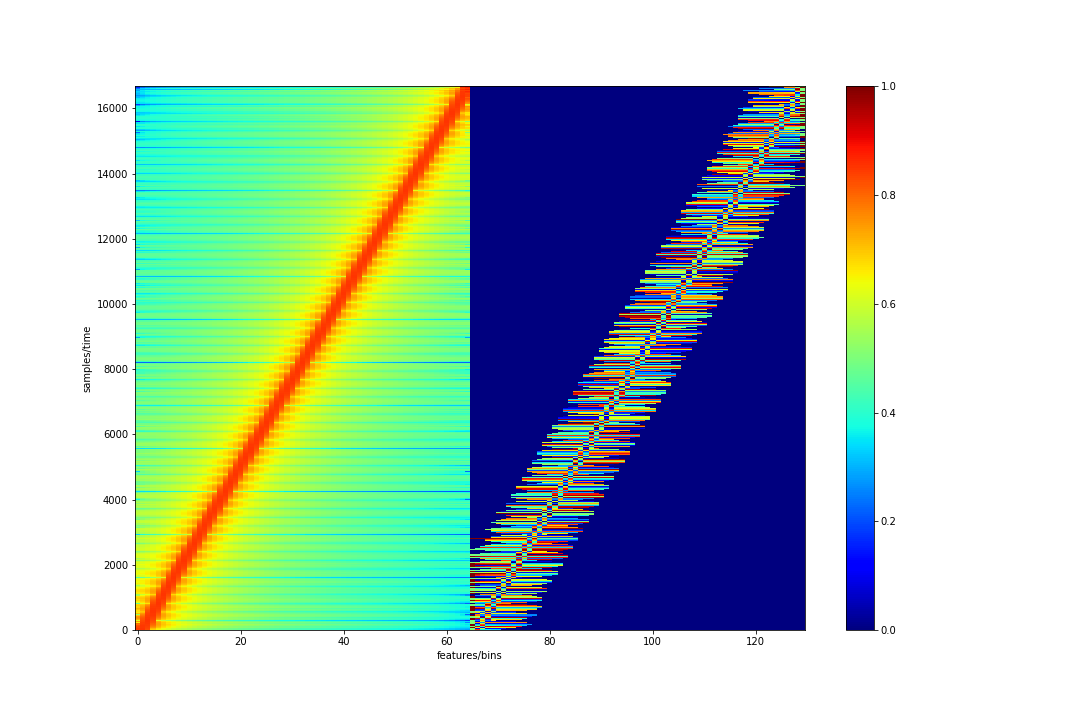
\includegraphics[width=0.7\linewidth]{dataExample.png}
				\caption{Training Data example. Amplitude and phase values concatenated. Sine sine sweep was used as input data. }	
			\end{figure}
		
	\end{frame}



	\begin{frame}{Pre-processing}
	To speed up learning and increase robustness, phase values can also be omitted completely 
	and generated by input signals or noise in sound generation phase after training.
	\end{frame}





	% \begin{frame}{Pre-processing}


	% 	\begin{figure}[ht]
	% 		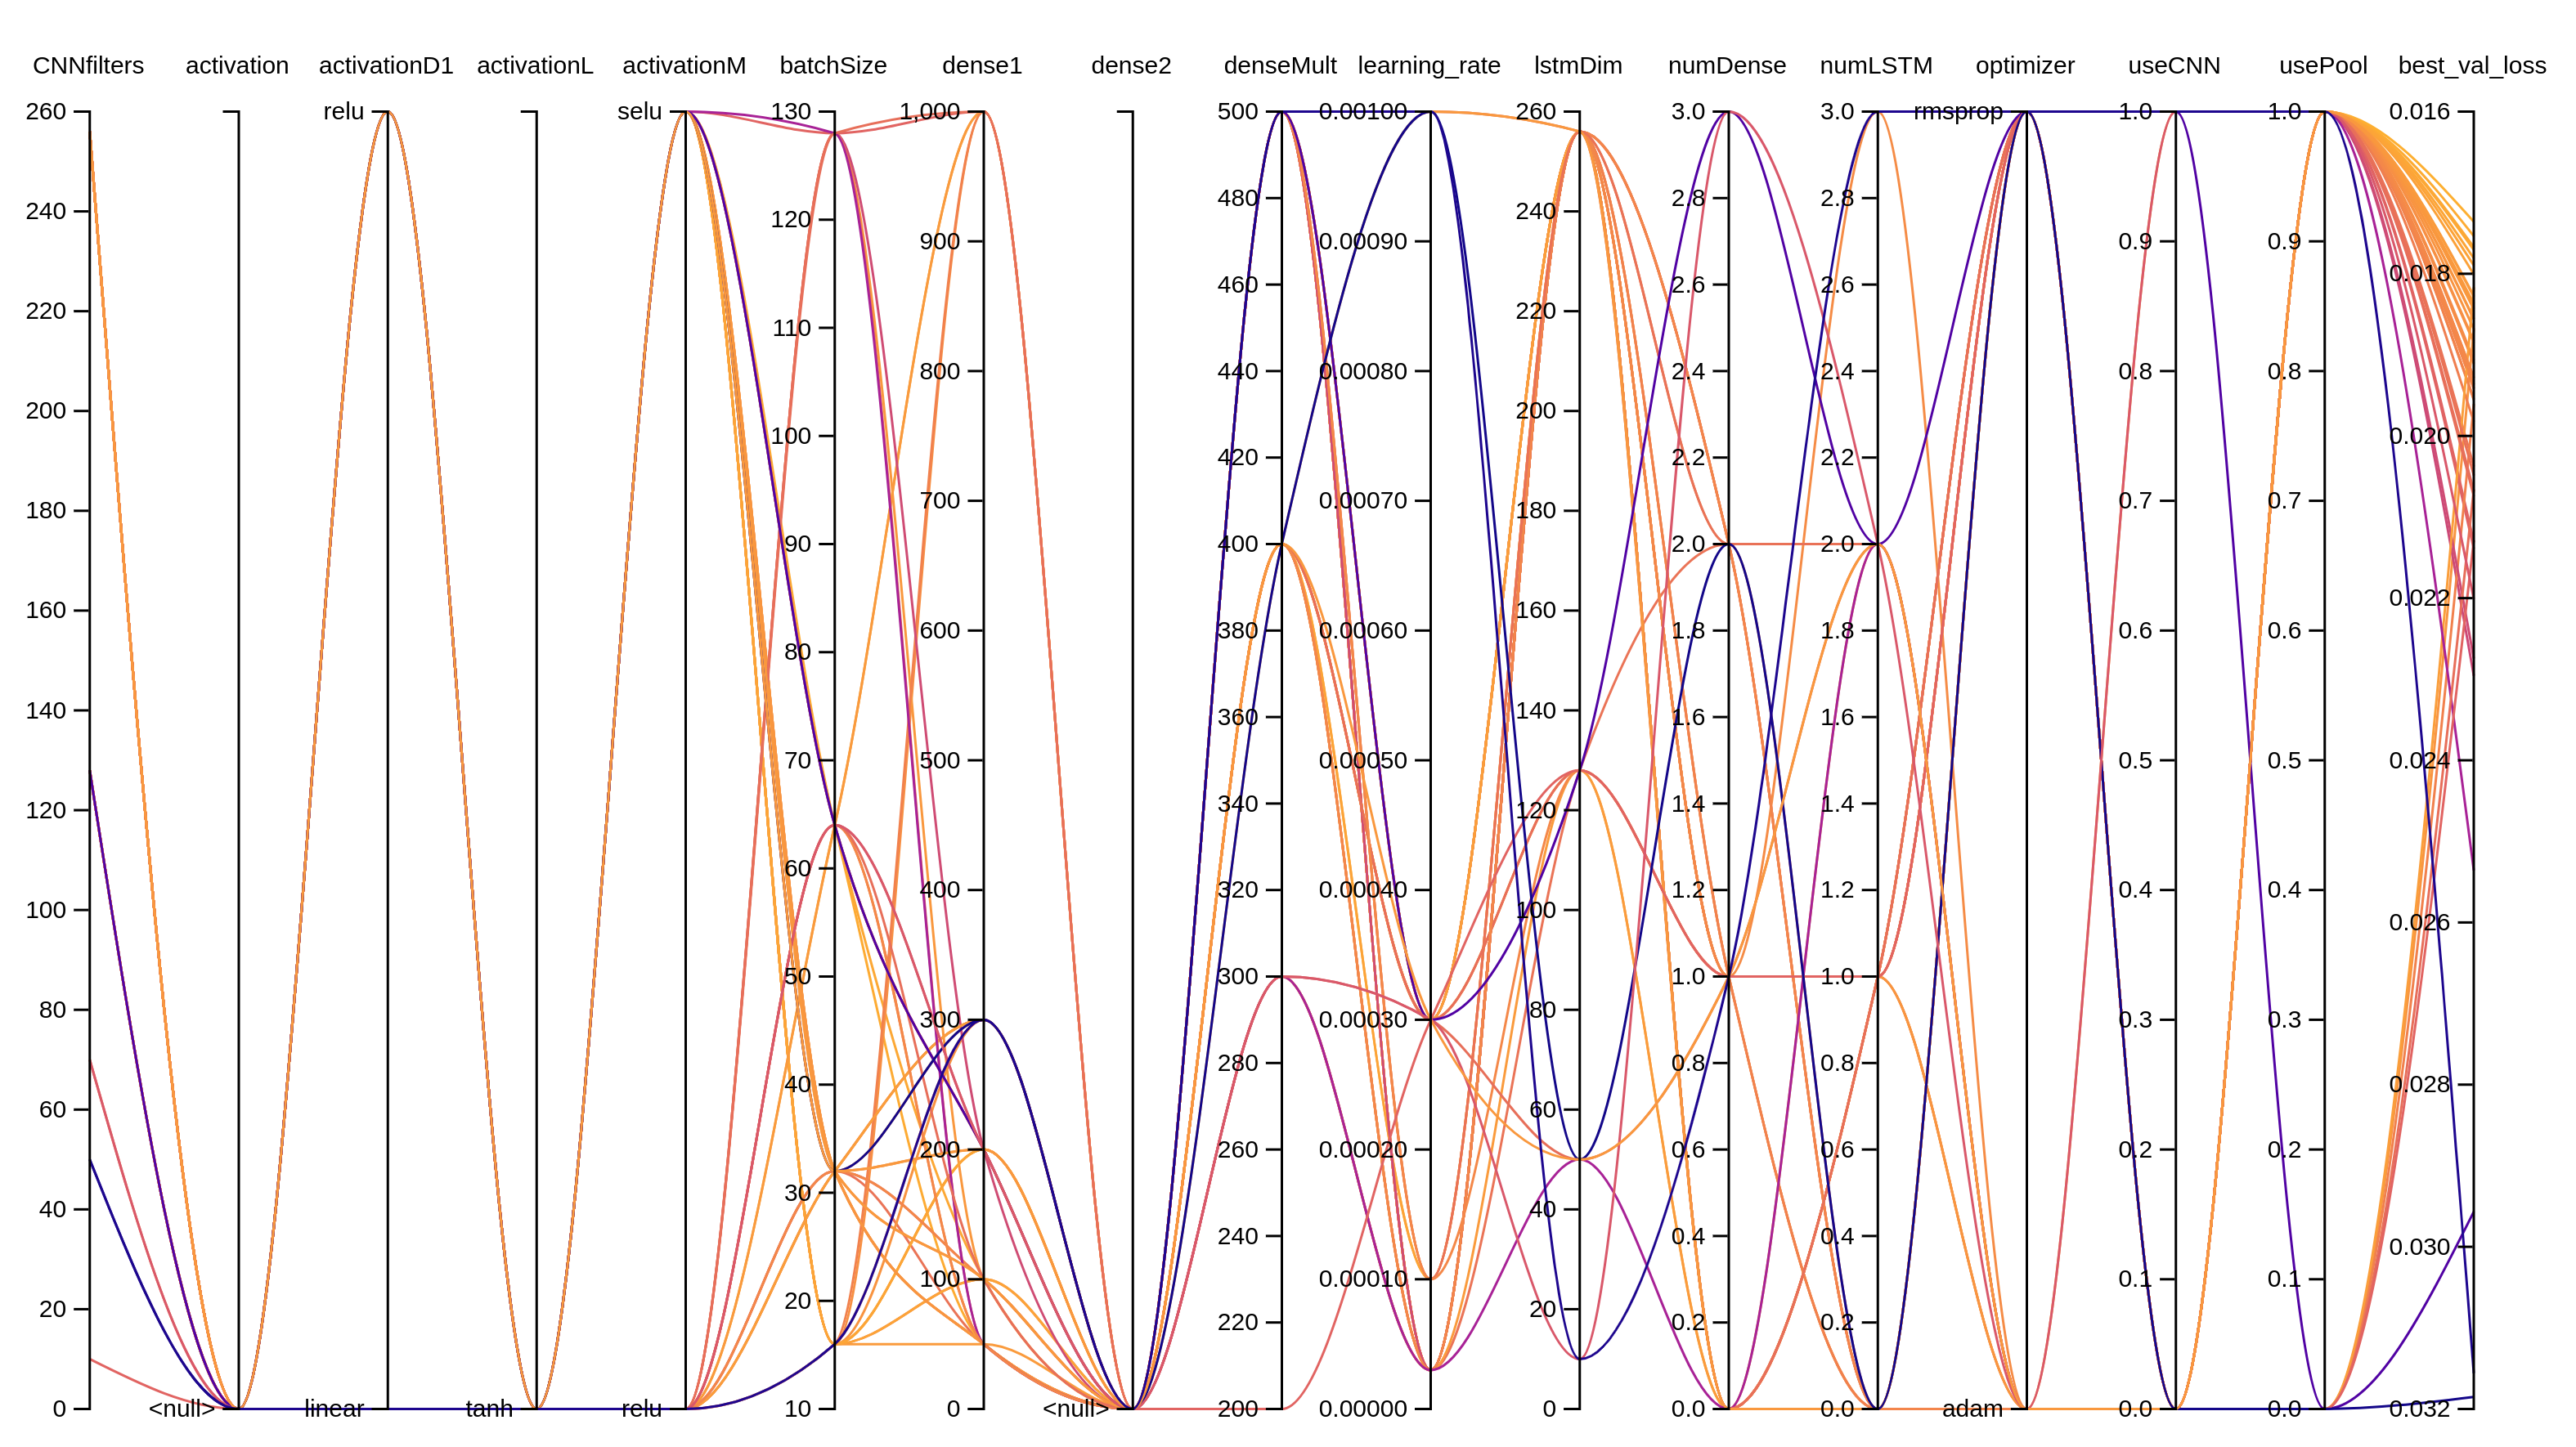
\includegraphics[width=1.\linewidth]{charts/Section-1-Panel-0-epgzprslg}
	% 		\end{figure}

	% 	% From the complex to amp/phase
	% 	% The obtained frames are further processed to facilitate the learining process:
	% 	% \begin{itemize}
	% 	% 	\item The complex valued Frames are converted to amplitude phase pairs:
	% 	% 	\item Tha amplitude values are  compressed
	% 	% 	\item Phase values of bins whose amplitude value is below a given hhreshold are omitted.
	% 	% \end{itemize}
		
	% \end{frame}


	\begin{frame}{Model Selection}



		\begin{figure}[ht]
			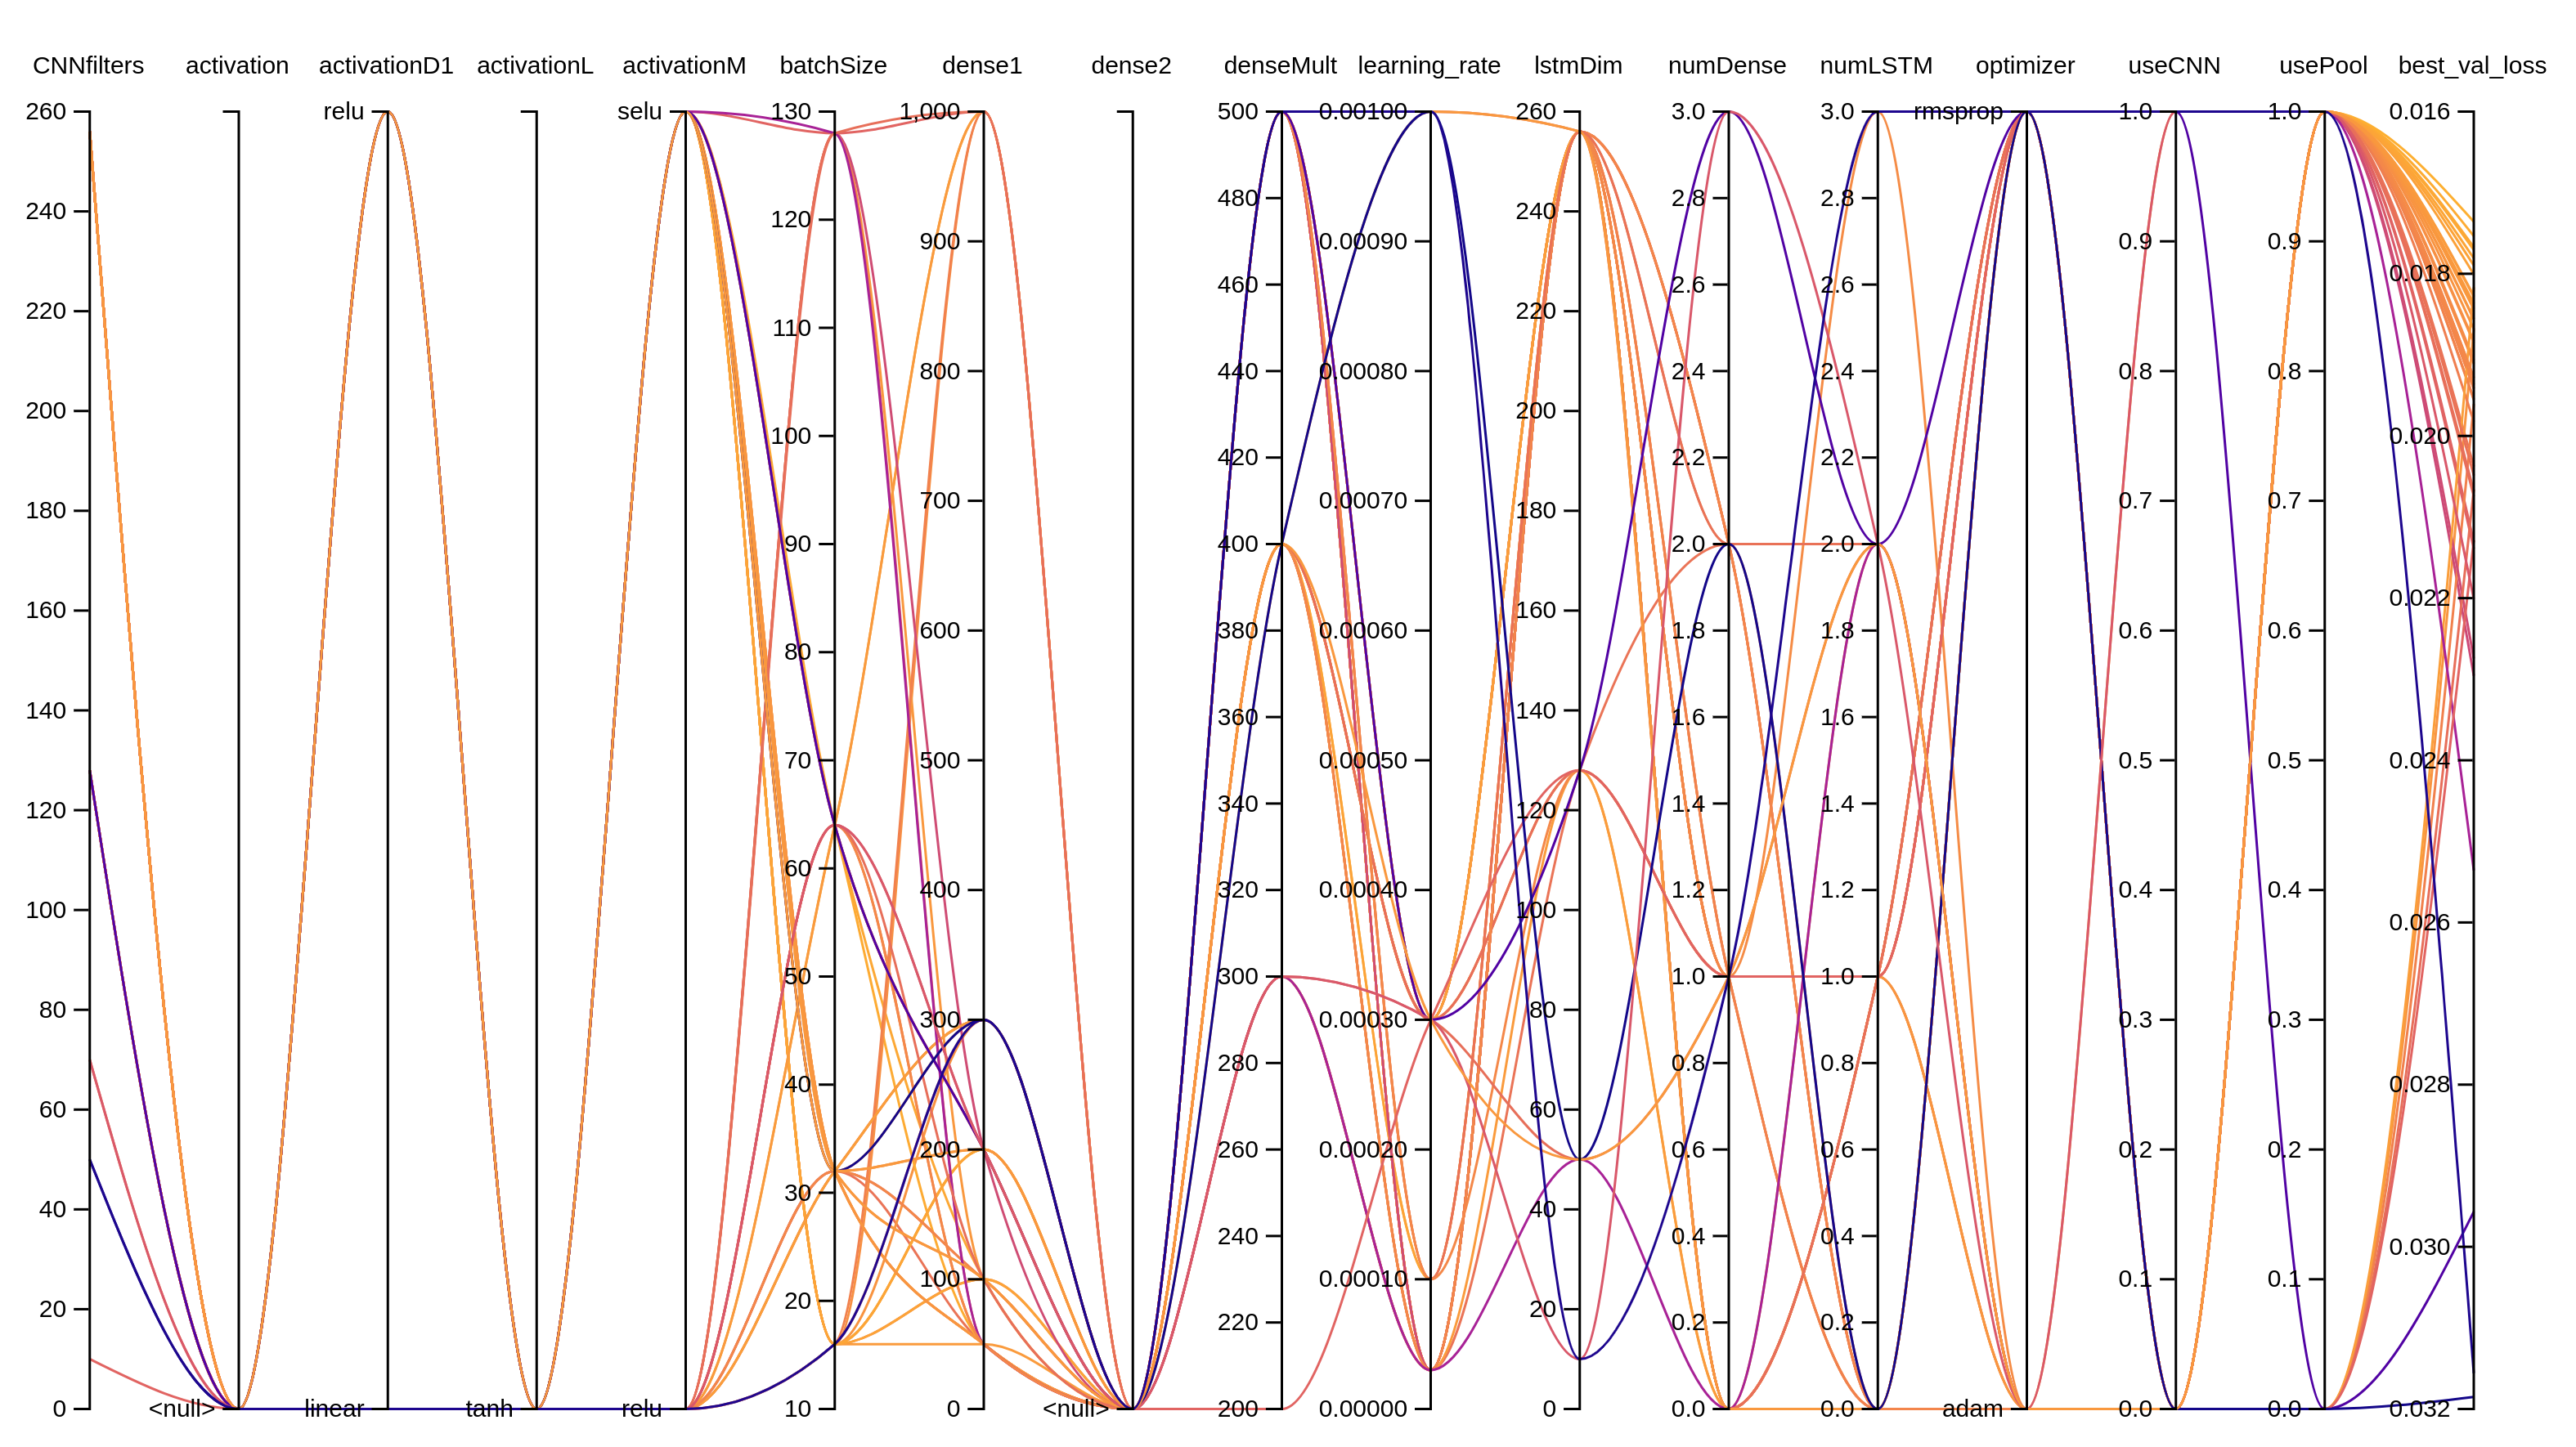
\includegraphics[width=1.\linewidth]{charts/Section-1-Panel-0-epgzprslg}
			\end{figure}



		% \begin{figure}
		% 	\begin{tabular}{cc}
		% 	\includegraphics[width=65mm]{it} &   \includegraphics[width=65mm]{it} \\
		% 	(a) first & (b) second \\[6pt]
		% 	\includegraphics[width=65mm]{it} &   \includegraphics[width=65mm]{it} \\
		% 	(c) third & (d) fourth \\[6pt]
		% 	\multicolumn{2}{c}{\includegraphics[width=65mm]{it} }\\
		% 	\multicolumn{2}{c}{(e) fifth}
		% 	\end{tabular}
		% \caption{caption}
		% \end{figure}
	\end{frame}


	\section{Results}
	\begin{frame}
		\begin{figure}[ht]
		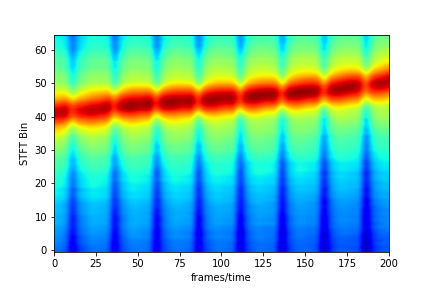
\includegraphics[width=0.6\linewidth]{modSinFbPredict.png}
		\caption{feedback prediction of a model trained with a modulated sine sweep.}
	\end{figure}
	\end{frame}



	\begin{frame}{Execution Speed}
		For a high performance Consumer Grade PC, Sampling rate 18kHz:\\

		around 15ms per 1024 bin FFT Frame. 
		This means around 270 samples @ 18 kHz(for model prediction only)


		% \begin{figure}[ht]
		% 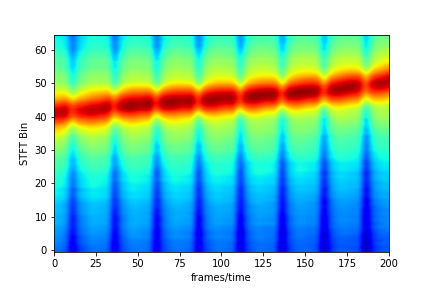
\includegraphics[width=0.6\linewidth]{modSinFbPredict.png}
		% \caption{feedback prediction of a model trained with a modulated sine sweep.}
	% \end{figure}
	\end{frame}




	% \begin{frame}{Sound example}

	% 	\includemedia[
	% 	  addresource=cello.mp3,
	% 	  flashvars={
	% 		source=cello.mp3
	% 	   &autoPlay=true
	% 	  }
	% 	]{\fbox{Play}}{APlayer.swf}
	% \end{frame}




	\section{Future Work}
	\begin{frame}
		A numer of augmentations to the presentaed sytem can be explored since the proposal is very general:
		\begin{itemize}
			\item Other architectures of the ANN
			\item Explore different encodings for different aethetical results and arttifacts
			\item Explore 'Convolutional Reverb'-like use cases
			\item Further explore different parametrozations (FFT Window length, number of input frames etc.)
			\item Robustness
			\item Real time implementation
		\end{itemize}

	\end{frame}




\end{document}


















